\noindent When this base version of the model is up and running, the second part of the research can start. The policy changes which are going to be analyzed are focused on the awareness of the citizens of Delft. \\
Delft has a population of more than 100.000 citizens \cite{Population2021}, with a population distribution as described in figure \ref{fig:Demographic_Pyramide}.

\begin{figure}[H]
    \centering
        \captionsetup{width=\linewidth}
        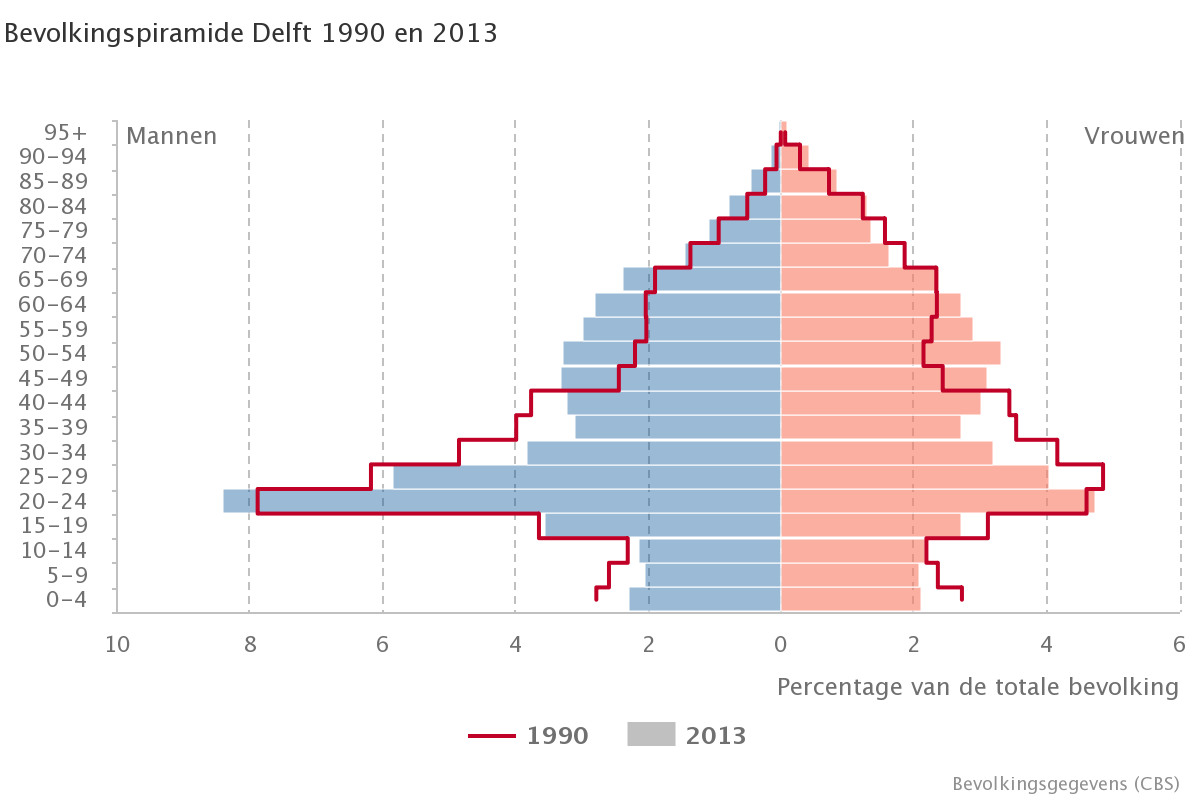
\includegraphics[width=0.7\linewidth]{Images/Piramide_Delft.png}
        \caption{Age pyramid of the citizens in Delft \cite{RIVM}}
    \label{fig:Demographic_Pyramide}
\end{figure}
\noindent The different age in this graph, means also a different perspective on waste recycling. (\textbf{FIND REFERENCE}).

\noindent To determine how much waste the municipality in Delft produces we assume that citizens in Delft produce the same amount per household as the average in the Netherlands. The Netherlands produces 1650 Kton of plastic waste